% !TEX root = epifanov_solid_state_physics.tex
%!TEX TS-program = pdflatex
%!TEX encoding = UTF-8 Unicode


\chapter[Bonding. The Internal Structure of Solids]{Bonding.\\The Internal Structure of Solids}\label{chap:1}
\chaptermark{Bonding. The Internal Structure of Solids}

Matter can exist in the solid state only because there are forces of interaction acting between the structural particles when the latter are brought sufficiently close together. For the solid to have a stable structure the forces of interaction between the particles should be of two types: of attraction, to prevent the particles from moving away from each other, and of repulsion, to prevent the particles from merging.

Let us discuss briefly the nature of these forces.

\section{The van der Waals forces}\label{sec:1_1}

The most general type of bond existing between any two atoms, or molecules, is due to van der Waals forces. Those forces were first introduced to explain the equation of state of real gases, the \textit{van der Waals equation}:
\begin{equation}\label{eq:1_1}
	\parenthesis{p + \frac{a}{V^2}}(V - b) = RT
\end{equation}

\noindent
where the correction terms $a/V^2$ and $b$ account, respectively, for the effect of the forces of attraction and repulsion acting between the molecules of a real gas. These forces manifest themselves in an almost ideal form in the interaction between the molecules with saturated chemical bonds (\ce{O2}, \ce{H2}, \ce{N2}, \ce{CH4}, etc.), as well as between the atoms of inert gases, making possible their existence in the liquid and solid states.

As a general case, the van der Waals bond is made up of the dispersion, orientational and induction interactions. Let's consider them separately.

\textbf{Dispersion interaction.} Consider the simplest example of two interacting helium atoms shown in \fig{1_1}. The electron density distribution in a helium atom is spherically symmetrical and for this reason its electric moment is zero. But this means only that the average electric moment of the atom is zero. At every moment of time the electrons occupy particular points in space, thereby creating instantaneous rapidly changing electric dipoles. When two helium atoms are brought together, the motion of their electrons becomes correlated and this leads to the forces of interaction. The forces can be of two types. If the motion of the electrons is correlated, as shown in \fig{1_1}(a), the instantaneous dipoles attract each other; if the correlation is as shown in \fig{1_1}(b), the resulting interaction is repulsion. Since the realization of the arrangement of \fig{1_1}(a) leads to a reduction in the energy of the system, this arrangement is more probable and is realized more frequently. This is in effect the cause of the constantly existing force of attraction between helium atoms.

\begin{figure}[t]
	\begin{center}
		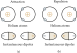
\includegraphics[scale=1]{figures/ch_01/fig_1_1.pdf}
		\caption[]{Dispersion interaction. The interaction between helium atoms is due to the correlation in the motion of electrons resulting in the appearance of instantaneous dipoles: (a) --- correlation resulting in attraction; (b) --- correlation resulting in repulsion.}
		\label{fig:1_1}
	\end{center}
	\vspace{-0.7cm}
\end{figure}

The bonds discussed above that owe their existence to a correlation in motion of the electrons in adjacent atoms are termed \textit{dispersion forces}. They were first calculated by F. London in 1930. The calculation was based on the following model: the instantaneous electric dipole of one atom causes the other atom to be polarized and it becomes an induced dipole leading to the realization of the arrangement in \fig{1_1}(a), which corresponds to attraction. The calculation had as its final result the following expression for the energy of the dispersion interaction of two particles:
\begin{equation}\label{eq:1_2}
	\ab{U}{d} = - \frac{3}{4}\frac{\alpha^2 \ab{E}{exc}}{r^6}
\end{equation}

\noindent
where $\alpha$ is the polarizability of the particles\footnote{Let us recall the physical meaning of $\alpha$. The charges in the molecule are displaced under the action of an external field of intensity $\mathscr{E}$. This leads to a dipole moment $M$ proportional to $\mathscr{E}: M = \alpha\mathscr{E}$, the proportionality factor $\alpha$ being the \textit{polarizability} of the molecule.}, $\ab{E}{exc}$ their energy of excitation, and $r$ the distance between them.

\textbf{Orientational interaction.} Should the molecules possess a constant dipole moment $M$, that is, should they be polar molecules, an electrostatic interaction would be established between them tending to arrange the molecules in a strict order (\fig{1_2}), since that order corresponds to the minimum energy of the system. The correct orientation of the molecules is disturbed by thermal motion. Therefore, the energy of the system due to the mutual orientation of the molecules is strongly dependent on temperature. At low temperatures, when the orientation of the molecules is perfect, the interaction energy is determined from the expression
\vspace{-12pt}
\begin{equation}\label{eq:1_3}
	\ab{U}{or} = - \frac{M^2}{2\pi\varepsilon_0 r^3}
\end{equation}

\noindent
where $r$ is the distance between the molecules, and $\varepsilon_0$ the permittivity of free space.

In the high temperature range the energy of interaction of polar molecules, as had been demonstrated by W. H. Keesom, is of the following form:
\begin{equation}\label{eq:1_4}
	\ab{U}{or} = - \frac{M^4}{24\pi^2\varepsilon_0^2 \ab{k}{B} T r^6}.
\end{equation}

\noindent
where $\ab{k}{B}$ is the Boltzmann constant and  $T$ the temperature.

The type of interaction discussed above is termed \textit{orientational interaction}.

\begin{figure}[t]
	\begin{minipage}[t]{0.48\linewidth}
		\begin{center}
			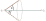
\includegraphics[scale=0.95]{figures/ch_01/fig_1_2.pdf}
			\caption[]{Orientational interaction of polar molecules.}
			\label{fig:1_2}
		\end{center}
	\end{minipage}
	\hfill{ }%\hspace{-0.1cm}
	\begin{minipage}[t]{0.48\linewidth}
		\begin{center}
			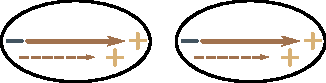
\includegraphics[scale=0.95]{figures/ch_01/fig_1_3.pdf}
			\caption[]{Induction interaction of molecules (dashed lines show the induced dipoles).}
			\label{fig:1_3}
		\end{center}
	\end{minipage}
\vspace{-0.3cm}
\end{figure}

\textbf{Induction interaction.} Lastly, in case of polar molecules of high polarizability an induced moment due to the action of the field of constant dipoles may be established (\fig{1_3}; the induced dipoles are shown by dashed lines). The energy of mutual attraction due to the interaction of the rigid dipole of the first molecule and the induced dipole of the second molecule, as has been shown by Debye, is independent of temperature and is given by the expression
\begin{equation}\label{eq:1_5}
	\ab{U}{in} = - \frac{\alpha M^2}{8\pi\varepsilon_0^2}\frac{1}{r^6}
\end{equation}

\noindent
where, as before, $M$ is the constant dipole moment of the molecule, and $\alpha$ its polarizability.

Such interaction is termed \textit{induction}, or \textit{deformation}, interaction.

In general, when two molecules are brought close together all three types of interaction may be established, the interaction energy being the sum of the energies of the dispersion ($\ab{U}{d}$), orientational
($\ab{U}{or}$), and induction ($\ab{U}{in}$) types of interaction:
\begin{equation*}
	U = \ab{U}{d} + \ab{U}{or} + \ab{U}{in}.
\end{equation*}

Table \ref{table:1_1} shows the relative magnitude (in percent) of each of those components of the total bonding energy for water, ammonia, hydrogen chloride and carbon monoxide. The data presented in Table \ref{table:1_1} show the induction interaction for all the substances to be weak. Three quarters or a half of the bond energy in substances made up of polar molecules is due to the energy of orientational interaction; while in materials made up of nonpolar molecules almost all of the bond energy is due to the dispersion interaction.

\begin{table}[!b]
	\renewcommand{\arraystretch}{1.2}
	\caption{}
	\vspace{-0.6cm}
	\label{table:1_1}
	\begin{center}\resizebox{0.84\linewidth}{!}{
			\begin{tabular}{lccc}
				\toprule[1pt]
				\multirow{2}{*}{\textbf{Substance}} & \multicolumn{3}{c}{\textbf{Type of interaction}}\\
				\cline{2-4}
				& \textbf{Dispersion} & \textbf{Induction} & \textbf{Orientational}\\
				\midrule[0.5pt]\midrule[0.5pt]
				Water & $19$ & $4$ & $77$\\
				Ammonia & $50$ & $5$ & $45$\\
				Hydrogen chloride & $81$ & $4$ & $15$\\
				Carbon monoxide & $100$ & &\\
				\bottomrule[1pt]
			\end{tabular}
	}\end{center}
\end{table}

Table \ref{table:1_2} shows the values of the bond energy for some molecular crystals held together by van der Waals forces.

\begin{table}[!b]
	\renewcommand{\arraystretch}{1.2}
	\caption{}
	\vspace{-0.6cm}
	\label{table:1_2}
	\begin{center}\resizebox{0.58\linewidth}{!}{
			\begin{tabular}{lc}
				\toprule[1pt]
				\textbf{Substance} & $\ab{U}{b}, \bracket{\SI{e3}{\joule\per\mole}}$\\
				\midrule[0.5pt]\midrule[0.5pt]
				Neon (\ce{Ne}) & $1.90$ \\
				Argon (\ce{Ar}) & $8.40$\\
				Nitrogen (\ce{N2}) & $6.60$\\
				Carbon monoxide (\ce{CO}) & $8.40$\\
				Oxygen (\ce{O2}) & $8.20$\\
				Methane (\ce{CH4}) & $10.8$\\
				\bottomrule[1pt]
			\end{tabular}
	}\end{center}
\end{table}

\section{The ionic bond}\label{sec:1_2}

Atoms that occupy places in the Mendeleev periodic table next to inert gases tend to assume the electronic configuration of these gases either by giving away or accepting electrons. The valence electron of alkali metals, which immediately follow the inert gases, moves outside the closed shell and is only weakly connected with the nucleus. The halides, which immediately precede the inert gases, lack one electron to complete a stable shell characteristic of an inert gas. Therefore, they exhibit high affinity to an excess electron.

Such atoms, that is, typical metals and halides, are bonded in the following way. First a recharging of the atoms takes place. The electron from the metal moves over to the halide. This turns the metal atom into a positively charged ion and the haloid atom into a negatively charged one. These ions interact according to the Coulomb law as two opposite charges. Such a bond became known as an \textit{ionic bond}.

The energy of attraction of two ions separated by the distance $r$ is
\begin{equation}\label{eq:1_6}
	\ab{U}{att} = - \frac{q^2}{4\pi\varepsilon_0 r}
\end{equation}

\noindent
where $q$ is the charge of the ions.

\begin{figure}[t]
	\begin{center}
		\includegraphics[scale=0.95]{figures/ch_01/fig_1_4.pdf}
		\caption[]{Dependence of energy of interacting ions on the distance between them: $1$ --- energy of attraction, $2$ --- energy of repulsion, $3$ --- total energy of interaction.}
		\label{fig:1_4}
	\end{center}
	\vspace{-0.7cm}
\end{figure}

The curve $1$ in \fig{1_4} shows the dependence of $\ab{U}{att}$ on $r$. As $r$ decreases the absolute value of the energy increases monotonically, tending to infinity as $r\to 0$. The force of attraction tends to bring the ions together as close as possible. This, however, is
prevented by the forces of repulsion, which begin to make themselves felt at small distances and rise very rapidly with the decrease in distance. The repulsion energy $\ab{U}{rep}$ is shown in \fig{1_4} by the curve $2$. Max Born and other scientists expressed the repulsion energy in the form
\begin{equation}\label{eq:1_7}
	\ab{U}{rep} = \frac{B}{r^n}
\end{equation}

\noindent
where $B$ and $n$ are constants.

The resulting interaction energy of two ions is
\begin{equation}\label{eq:1_8}
	U = \ab{U}{rep} + \ab{U}{att} = \frac{B}{r^n} - \frac{q^2}{4\pi\varepsilon_0 r}.
\end{equation}

This energy is shown in \fig{1_4} by the curve $3$ which has a minimum at $r=r_0$; the depth of this minimum determines the bond energy $\ab{U}{b}$, and $r_0$ determines the distance between the ions in the molecule. Making use of the fact that in equilibrium (at $r=r_0$) the force of attraction, $\ab{F}{att}=-(\diffin{\ab{U}{att}}{r})_{r=r_0}$, equals the force of repulsion, $\ab{F}{rep}=-(\diffin{\ab{U}{rep}}{r})_{r=r_0}$, we can easily express \eqref{eq:1_8} as
\begin{equation}\label{eq:1_9}
	\ab{U}{b} = - \frac{q^2}{4\pi\varepsilon_0 r_0} \parenthesis{1 - \frac{1}{n}}.
\end{equation}

The energy of the lattice made up of $N$ such molecules is
\begin{equation}\label{eq:1_10}
	\ab{U}{lattice} = - NA \frac{q^2}{4\pi\varepsilon_0 r_0} \parenthesis{1 - \frac{1}{n}}
\end{equation}

\noindent
where $A$ is the \textit{Madelung constant}, which takes account of the energy of interaction of the given molecule with all its neighbouring molecules in the crystal.

Table \ref{table:1_3} shows by way of an example the experimental values of the bond energy of some ionic crystals and its values calculated with the aid of \eqref{eq:1_10}. The discrepancies do not exceed $1$-$2$ percent, which is proof of good agreement between theory and experiment.

\begin{table}[!b]
	\renewcommand{\arraystretch}{1.2}
	\caption{}
	\vspace{-0.6cm}
	\label{table:1_3}
	\begin{center}\resizebox{0.68\linewidth}{!}{
			\begin{tabular}{lcc}
				\toprule[1pt]
				\multirow{2}{*}{\textbf{Crystal}} & \multicolumn{2}{c}{$\ab{U}{b}, \bracket{\SI{e3}{\joule\per\mole}}$}\\
				\cline{2-3}
				& \textbf{Experiment} & \textbf{Theory}\\
				\midrule[0.5pt]\midrule[0.5pt]
				Sodium chloride (\ce{NaCl}) & $752$ & $754$\\
				Potassium iodine (\ce{KI}) & $650$ & $630$\\
				Rubidium bromide (\ce{RbBr}) & $635$ & $645$\\
				Caesium iodine (\ce{CsI}) & $595$ & $585$\\
				\bottomrule[1pt]
			\end{tabular}
	}\end{center}
\end{table}

\section{The covalent bond}\label{sec:1_3}

The ionic and van der Waals bonds are unable to account for the existence of such compounds as \ce{H2}, \ce{O2}, \ce{N2}, etc., as well as for bonds in atomic crystals of the diamond type. Evidently, atoms of one kind cannot form oppositely charged ions by changing the distribution of valence electrons, as was the case in the metal-halide interaction. On the other hand, the bond in the \ce{H2}, \ce{O2} and \ce{N2} molecules is much stronger than that which could be attributed to the van der Waals forces. For such compounds the role of the van der Waals forces is that of a small correction to the bond mainly responsible for the strength of the compounds. This bond became known as the \textit{covalent bond}.

Let us consider the nature of this type of bond using the hydrogen molecule as an example.

Suppose that two hydrogen atoms are at a rather great distance $r$ from one another. The atom A consists of the nucleus a and the electron $1$ and the atom B consists of the nucleus b and the electron $2$ (\fig{1_5}). Since the density of the electron cloud which describes the electron state in an atom falls off very rapidly as the distance from the nucleus increases, the probabilities to discover electron $1$ near nucleus b and electron $2$ near nucleus a are very small. Calculation shows that for $r\approx\SI{50}{\angstrom}$ each electron can visit the other nucleus on the average only once in \num{e12} years. Because of that atoms A and B may be regarded as isolated atoms and the energy of the system made up of such atoms may be taken to be equal to $2E_0$, where $E_0$ is the energy of the isolated atom in the ground state.

\begin{figure}[t]
	\begin{center}
		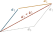
\includegraphics[scale=1]{figures/ch_01/fig_1_5.pdf}
		\caption[]{Calculating covalent bond between hydrogen atoms: A, B --- hydrogen atoms; a, b --- their nuclei; 1 --- electron of atom A; 2 --- electron of atom B; $\ab{r}{a$1$}, \ab{r}{b$2$}$ --- distances of electrons from their nuclei; $r_{12}$ --- distance between electrons; $\ab{r}{a$2$}$ --- distance of electron $2$ from nucleus a; $\ab{r}{b$1$}$ --- distance of electron $1$ from nucleus b; $r$ --- distance between nuclei.}
		\label{fig:1_5}
	\end{center}
	\vspace{-0.7cm}
\end{figure}

When the atoms are brought closer together, the probability of the electrons going over to nuclei other than their own increases. For $r\approx\SI{2}{\angstrom}$ the electron clouds begin to overlap noticeably and the transition frequency rises up to \SI{e14}{\per\second}. If the atoms are brought still closer together, the frequency of the electron exchange rises so that it becomes meaningless to speak of electron $1$ as belonging to the atom A and of electron $2$ as belonging to atom B. This corresponds to a new state that is not characteristic for a system made up of two isolated atoms. A remarkable property of this new state is that the electrons in it belong simultaneously to both nuclei, in other words, are \textit{collectivized}.

The collectivization of the electrons is accompanied by a change in the electron density distribution $\absolute{\psi}^2$ and in the energy of the system as compared to the total energy $2E_0$ of the isolated atoms. The lines $1$ in \fig{1_6} show the electron cloud density of the isolated atoms, the line $2$ shows the total density obtained by simple superposition of the electron clouds of isolated atoms, and the line $3$ the actual density distribution along the axis joining the nuclei a and b brought about by the collectivization of the electrons. The figure shows that the collectivization of the electrons results in the electron clouds being drawn into the space between the two nuclei: at a small distance from the nucleus outside this space the density of the clouds falls off, as compared with the density in isolated atoms, at the same time rising in the space between the nuclei above the sum of the densities of isolated atoms. The appearance of a state with an electron cloud of increased density that fills the space between the nuclei always results in a decrease in the system's energy and in the appearance of forces of attraction between the atoms. Speaking figuratively, we may say that the electron cloud formed in the space between the nuclei by a collectivized pair of electrons draws the nuclei together, striving to bring them as close together as possible.

\begin{figure}[t]
	\begin{center}
		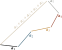
\includegraphics[scale=1]{figures/ch_01/fig_1_6.pdf}
		\caption[]{Electron density distribution in a system of two hydrogen atoms: $1$ --- electron density distribution in isolated hydrogen atoms, $2$ --- electron density resulting from simple overlapping of electron clouds of isolated atoms brought together to within a distance of $r$, $3$ --- actual electron density distribution in a hydrogen molecule.}
		\label{fig:1_6}
	\end{center}
	\vspace{-0.7cm}
\end{figure}

Such is the qualitative picture of the origin of the covalent bond. Quantitative calculations of the hydrogen molecule were first performed by W. H. Heitler and F. London in 1927. Those calculations have shown that a system consisting of two closely spaced atoms of hydrogen can have two energy values depending on the direction of the electron spins in the atoms:
\begin{equation}\label{eq:1_11}
	\ab{U}{s} = 2 E_0 + \frac{(K + A)}{(1 + S^2)}
\end{equation}

\noindent
when the spins are antiparallel, and
\begin{equation}\label{eq:1_12}
	\ab{U}{a} = 2 E_0 + \frac{(K + A)}{(1 - S^2)}
\end{equation}

\noindent
when the spins are parallel. Here $2E_0$ is the total energy of the two isolated atoms, $K$ is the \textit{energy of the electrostatic interaction} of the electrons with the nuclei, of the electrons with one another, and of the nuclei. Another name for it is \textit{Coulomb energy}. Its sign is negative. By $A$ we denote the \textit{energy of exchange interaction} due to the atoms exchanging electrons. This is the additional energy that appears as the result of the change in the electron density distribution in the process of the formation of the molecule. Its sign is negative and its absolute value is much larger than $K$ ($|A|\gg |K|$). $S$ is the \textit{overlap integral} whose value lies within the limits $0\leqslant S\leqslant 1$.

The state with the energy $\ab{U}{s}$ is termed \textit{symmetric} and with $\ab{U}{a}$ \textit{antisymmetric}. Since both $K$ and $A$ are negative and $S\leqslant 1$, the energy of the system in the symmetric state is less than the energy of two isolated atoms:
\begin{equation}\label{eq:1_13}
	\ab{U}{s} < 2 E_0.
\end{equation}

\noindent
This corresponds to the appearance of forces of attraction. Since the absolute value of the exchange energy $A$ is considerably greater than that of the Coulomb energy $K$ the decrease in the system's energy is mainly due to $A$. For this reason the force of attraction that appears between the atoms is termed the \textit{exchange force}.

For the same reason, that is, because $|A|\gg |K|$, the formation of the antisymmetric state leads to an increase in the system's energy. This corresponds to the appearance of repulsive forces.

Figure \ref{fig:1_7} shows the dependence of $\ab{U}{s}$ and $\ab{U}{a}$ on $r/a$, where $r$ is the distance between the atoms, and $a=\SI{0.529}{\angstrom}$ is the radius of the first Bohr orbit (the \textit{Bohr radius}). The zeroth energy level has been fixed at $2E_0$. Figure \ref{fig:1_7} shows that in the antisymmetric state the system's energy rises steadily as the atoms are brought closer together (curve $7$), this corresponding to the mutual repulsion of the atoms. Therefore a hydrogen molecule cannot be formed in such a state. In the symmetric state (curve $2$) the system's energy at first falls as the distance $r$ between the atoms decreases, attaining its minimum value at $r=r_0$.
As the distance $r$ decreases still further, the energy begins to rise because of the appearance of strong repulsive forces. The existence of a minimum on the potential energy curve makes the existence of a stable system of two hydrogen atoms, that is, a hydrogen molecule, possible. To destroy this system work must be performed equal to the depth of the potential well, $\ab{U}{b}$.

\begin{figure}[t]
	\begin{center}
		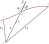
\includegraphics[scale=1]{figures/ch_01/fig_1_7.pdf}
		\caption[]{Interaction energy of two hydrogen atoms: $1$ --- antisymmetric state, $2$ --- symmetric state.}
		\label{fig:1_7}
	\end{center}
	\vspace{-0.7cm}
\end{figure}

Calculation provides the following values of $\ab{U}{b}$ and $r_0$: $\ab{U}{b}=\SI{4.37}{\electronvolt}, r_0=\SI{0.735}{\angstrom}$; the experimental values are $\ab{U}{b}=\SI{4.38}{\electronvolt}, r_0=\SI{0.753}{\angstrom}$. The agreement between theory and experiment
is quite good.

Table~\ref{table:1_4} shows the values of the bond energy for some covalent compounds---the molecules of \ce{H2}, \ce{N2}, \ce{O2}, \ce{CO}---and for diamond, silicon and germanium crystals in which the bonding is due to covalent forces.

\begin{table}[!b]
	\renewcommand{\arraystretch}{1.2}
	\caption{}
	\vspace{-0.6cm}
	\label{table:1_4}
	\begin{center}\resizebox{0.58\linewidth}{!}{
			\begin{tabular}{lc}
				\toprule[1pt]
				\textbf{Gas} & $\ab{U}{b}, \bracket{\SI{e5}{\joule\per\mole}}$\\
				\midrule[0.5pt]\midrule[0.5pt]
				Carbon monoxide (\ce{CO}) & $10.8$\\
				Nitrogen (\ce{N2}) & $9.50$\\
				Oxygen (\ce{O2}) & $5.00$\\
				Hydrogen (\ce{H2}) & $4.40$ \\
				Diamond (\ce{C}) & $6.80$\\
				Silicon (\ce{Si}) & $4.40$\\
				Germanium (\ce{Ge}) & $3.50$\\
				\bottomrule[1pt]
			\end{tabular}
	}\end{center}
\end{table}

Characteristic properties of the covalent bond, which distinguish it from the bonds of other types, are its \textit{saturability} and \textit{directionality}.

Saturability means that each atom can form covalent bonds only with a limited number of its neighbours. This means that each hydrogen atom can form covalent bonds only with one of its neighbours. The electron pair constituting such a bond has antiparallel spins and occupies one quantum cell. A third atom in this case instead of being attracted will be repelled.

The valence bond is formed in the direction of the greatest density of the electron cloud corresponding to the valence electrons. In this case there is maximum overlapping of the electron clouds of the bonding electrons, which implies that the valence bond is directional.

\section{The metallic bond}\label{sec:1_4}

There is a special group of substances, called metals, that occupy places at the beginning of every period of the Mendeleev table. The formation of the metallic bond cannot be explained by the presence of the ionic or the covalent bond. Indeed, the ionic bond appears only between atoms having different affinities to the additional electron, for instance, between the atoms of a metal and a halide. Evidently, such bond between kindred atoms of a metal having identical affinity to the electron is impossible. On the other hand, metallic atoms do not have enough valence electrons to form valence bonds with their nearest neighbours. For instance, the copper atom has one valence electron and can form a valence bond only with a single atom. But in the copper lattice every atom is surrounded by twelve neighbours with which it must be connected by lines of force. This points to the fact that in metals there is a special type of bonding known as the \textit{metallic bond}. Let us consider the nature of this bond.

In metallic atoms the external valence electrons are rather weakly coupled to the nucleus. In the liquid and solid states the atoms come so close together that the valence electrons are able to leave their respective atoms and wander throughout the lattice. This leads to an extremely homogeneous distribution of the negative charge in the crystal lattice. This conclusion is supported by direct experiments. Figure \ref{fig:1_8} shows an experimental curve of the electron density distribution between the sites of the aluminium lattice obtained by means of X-ray photography. Most part of the distance between the sites the electron concentration remains constant. Only quite close to the sites it rises sharply because of the presence of internal shells of the aluminium atoms.

\begin{figure}[t]
	\begin{center}
		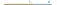
\includegraphics[scale=0.85]{figures/ch_01/fig_1_8.pdf}
		\caption[]{Electron density distribution in the aluminium lattice obtained by X-ray photography.}
		\label{fig:1_8}
	\end{center}
	\vspace{-0.7cm}
\end{figure}

In the lattice of a metal the bond is due to the interaction of the positive ions with the electron gas. The electrons moving between the ions compensate the forces of repulsion existing between the positively charged ions and draw them closer together. As the distance between the ions becomes smaller the density of the electron gas rises and this leads to an increase in the force drawing the ions together. On the other hand, in this case the repulsive forces acting between the ions tend to move them away from each other. When the distance between the ions becomes such that the forces of attraction are compensated by the forces of repulsion, a stable lattice is formed.

It appears that the metallic bond is somewhat similar to the valence bond, since they are both based on the collectivization of external valence electrons. However, in case of the valence bond only atoms that form pairs of nearest neighbours take part in the collectivization of electrons, and the respective electrons always remain between the atoms. In case of the metallic bond all atoms of the crystal take part in the collectivization of electrons, and the collectivized electrons are no longer localized near their respective atoms but move freely inside the lattice.

\section{The hydrogen bond}\label{sec:1_5}

The \textit{hydrogen bond} is formed between an atom of hydrogen and an extremely electronegative atom, for instance, an atom of oxygen, fluorine, nitrogen, chlorine. Such an atom attracts the bonding electrons and becomes negatively charged; the hydrogen atom after losing the bonding electron assumes a positive charge. The hydrogen bond is a result of electrostatic attraction of those charges.

\begin{figure}[t]
	\begin{center}
		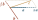
\includegraphics[scale=0.85]{figures/ch_01/fig_1_9.pdf}
		\caption[]{Hydrogen bond between water molecules.}
		\label{fig:1_9}
	\end{center}
	\vspace{-0.7cm}
\end{figure}

As a typical example we may cite the hydrogen bond between molecules of water (\fig{1_9}). The \ce{O-H} bond between an oxygen atom of one molecule and a hydrogen atom of another behaves as a tiny dipole with a $-\delta$ charge on the oxygen atom and a $+\delta$ charge on the hydrogen atom. The force of attraction between those charges is the cause of the hydrogen bond shown by dots in \fig{1_9}. The attraction is enhanced by the small dimensions of the hydrogen atom that enable it to come close to the electronegative atom. Still, this distance $r_{\ce{OH}}=\SI{2.76}{\angstrom}$ is much greater than the radius of the covalent bond \ce{H-O}, $r_0$, in the water molecule itself, which is equal to \SI{0.96}{\angstrom}. This is quite natural since the energy of the covalent bond is about an order of magnitude higher than that of the hydrogen bond. Its value for water is \SIrange{21e3}{25e3}{\joule\per\mole}.

The hydrogen bond is the cause of association of molecules of liquids (water, acids, spirits, etc.), which results in greater viscosity, higher boiling point, abnormal thermal expansion, etc. Water may serve best to illustrate this. Should there be no hydrogen bonds between the molecules of water, its boiling point at atmospheric pressure would be not $+\SI{100}{\degreeCelsius}$ but $-\SI{80}{\degreeCelsius}$ and its viscosity would be lower by almost an order of magnitude. When water is heated above \SI{0}{\degreeCelsius}, the hydrogen bond is destroyed. Since the hydrogen bond is responsible for the loose structure of associated complexes, in which the water molecules are rather far apart (\SI{2.76}{\angstrom}), the destruction of such a loose structure should result in an increase in the density of water. On the other hand, an increase in the temperature of water and a corresponding increase in the intensity of thermal motion of its molecules should lead to thermal expansion and a decrease in its density. Experiment shows that in the temperature range \SIrange{0}{4}{\degreeCelsius} the first factor---the increase in density due to the disruption of the hydrogen bonds---is the prevalent one. Because of that within this range the density of water rises upon heating. Above \SI{4}{\degreeCelsius} the other factor---thermal expansion---prevails. This is why when water is heated above \SI{4}{\degreeCelsius} its density decreases, as is the case with other (normal) liquids.

\section{Comparison between bonds of various kinds}\label{sec:1_6}

The van der Waals bond is the most universal one. It exists in all cases without exception. At the same time this is the weakest, having an energy of the order of \SI{e4}{\joule\per\mole}. Ideally, it operates between neutral atoms, or molecules, with closed inner electron shells. Specifically, the van der Waals forces are responsible for the existence of the liquid and solid states of inert gases, hydrogen, oxygen, nitrogen and many other organic and inorganic compounds. They also, as we will see later, form bonds in many of the molecular valence crystals. Because of low energy values of the van der Waals bond all structures based on it are unstable, volatile and have low melting points.

The ionic bond is a typical chemical bond very frequent among the inorganic compounds such as metal-halide compounds, metallic oxides, sulfides and other polar compounds. The ionic bond is also a feature of numerous intermetallic compounds (carbides, nitrides, selenides, etc.). The energy of the ionic bond is much higher than that of the van der Waals bond and may be as high as \SI{e6}{\joule\per\mole}. Because of that solids based on the ionic bond have high sublimation heat values and high melting points.

The covalent bond is extremely widespread among organic compounds, but is also present in inorganic compounds, in some metals and in numerous intermetallic compounds. This bond is responsible for the existence of valence crystals of the diamond, germanium and other types, as will be discussed below. The energy of the covalent bond is also high ($\sim\!\SI{e6}{\joule\per\mole}$), which stems from the fact that the solids with this type of bond have high melting points and high heats of sublimation.

The metallic bond formed as a result of the collectivization of the valence electrons is characteristic of typical metals and numerous intermetallic compounds. The order of magnitude of the energy of this type of bond is comparable to that of the energy of covalent bond.

Lastly, the hydrogen bond, although relatively weak, still plays an important part in nature.

It should be pointed out that in real solids no types of bonds discussed above ever exist purely by themselves. Practically, there is always a superposition of two types of bonds or more. One of them, as a rule, plays a dominant part in determining the structure and the properties of the solid.

\section{Forces of repulsion}\label{sec:1_7}

For the formation of a stable system of interacting atoms or molecules, together with forces of attraction there should be forces of repulsion, which would prevent the complete merging of the particles.

The origin of the forces of repulsion is first of all the interaction of the nuclei each of which carries a considerable positive charge. The energy of this interaction, $\ab{U}{rep}'$ depends on the distance between the nuclei and on the degree of screening by their internal electron shells.

The following expression for $\ab{U}{rep}'$ may be obtained from quantum mechanical calculations:
\begin{equation}\label{eq:1_14}
	\ab{U}{rep}' \propto e^{-r/a}
\end{equation}

\noindent
where $r$ is the distance between the nuclei, and $a=\SI{0.529}{\angstrom}$ the Bohr radius.

This dependence of $\ab{U}{rep}'$ on $r$ determines the nature of the forces of repulsion: they attain enormous values at short distances and
fall off abruptly as $r$ increases. For instance, when the distance between a proton and a hydrogen atom decreases from $r=2a$ to $r=a/2$ ($4$ times), the repulsive energy increases almost $300$-fold.

The repulsive forces due to the interaction of the nuclei play a dominant role when light atoms, whose nuclei are rather poorly screened by the electron shells, are brought together. In all other cases the dominant part is played by repulsion due to the overlapping of closed electron shells of the atoms being brought together. Consider by way of an example the interaction between a chlorine ion with a closed \enlevel{3}{p}{} shell and a sodium ion with a closed \enlevel{2}{p}{} shell. When the ions are brought together to a distance at which the \enlevel{3}{p}{} and \enlevel{2}{p}{} shells overlap, the number of electrons in each of them begins to exceed that which is compatible with the Pauli exclusion principle. Because of that some of the electrons are forced to go to higher energy levels (for instance, \enlevel{3}{d}{} or \enlevel{4}{s}{}). This results in an increase in the system's energy and, consequently, in the appearance of forces of repulsion. Quantum mechanical calculations show the energy of such repulsion to have an exponential dependence on the distance, as well:
\begin{equation}\label{eq:1_15}
	\ab{U}{rep}'' \propto e^{-r/\rho}
\end{equation}

\noindent
where $\rho$ is a constant usually obtained experimentally.

Often the repulsion energy is expressed in the form \eqref{eq:1_7}. This expression gives a less steep decline of $\ab{U}{rep}$ with the increase in $r$ and is less consistent with experiment than \eqref{eq:1_14} or \eqref{eq:1_15} but is nevertheless widely used by researchers.

\begin{figure}[t]
	\begin{center}
		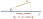
\includegraphics[scale=0.95]{figures/ch_01/fig_1_10.pdf}
		\caption[]{Interaction between approaching particles: (a) --- interaction forces, $1$ --- force of attraction, $2$ --- repulsive force, $3$ --- resultant force; (b) --- interaction energy.}
		\label{fig:1_10}
	\end{center}
	\vspace{-0.7cm}
\end{figure}

\section{Crystal lattice}\label{sec:1_8}

No matter what the origin of forces appearing when particles are brought together is, their general nature is the same [\fig{1_10}(a)]: at comparatively large distances forces of attraction $\ab{F}{att}$ increase rapidly as the distance between the particles decreases (curve $1$); at small distances forces of repulsion $\ab{F}{rep}$ come into being and with a further decrease in $r$ they increase much more rapidly than $\ab{F}{att}$ (curve $2$). At the distance $r=r_0$ the repulsive forces counterbalance the forces of attraction, the resultant force of interaction $F$ vanishes (curve $3$), and the energy attains its minimum value $\ab{U}{b}$ [\fig{1_10}(b)]. Because of this the particles brought together to a distance $r_0$ are in a state of stable equilibrium. By the same reason the free particles should arrange themselves in a strict
order at a distance $r_0$ from one another thus forming a body with a regular internal structure---a crystal. Such a structure will remain stable until the absolute value of the bond energy remains greater than the energy of thermal motion of the particles. The particles constituting
the crystal cannot freely leave their equilibrium sites because this involves an increase in their energy and leads to the appearance of forces tending to return them to their equilibrium sites. One may say that the particles are fixed in their equilibrium sites. The only form of motion allowed to them are random vibrations around their equilibrium sites.

To describe the regular internal structure of crystals one may conveniently use the concept of the crystal lattice. There are lattices of two types---the translational Bravais lattice and the lattice with a basis.

\textbf{Bravais lattice.} From the geometrical point of view a regular periodic arrangement of particles may be described with the aid of a translation. Figure \ref{fig:1_11}(a) shows a lattice obtained with the aid of translation of a particle along the three axes: $0X$ over the sections $a, 2a, 3a,\ldots, ma, \ldots$; $0Y$ over the sections $b, 2b, 3b, \ldots, nb, \ldots$; $0Z$ over the sections $c, 2c, 3c, \ldots, pc, \ldots$ ($m, n, p$ are integers). The position of any particle in this lattice is described by the vector
\begin{equation}\label{eq:1_16}
	\vec{r} = m\vec{a} + n\vec{b} + p\vec{c}.
\end{equation}

\noindent
The vectors $\vec{a}, \vec{b}, \vec{c}$ are termed the \textit{translation vectors} and their numerical values the \textit{translation periods}.

\begin{figure}[t]
	\begin{center}
		
\includegraphics[scale=1]{figures/ch_01/fig_1_11.pdf}
		\caption[]{Crystal lattice: (a) --- Bravais lattice, (b) --- unit cell of Bravais lattice.}
		\label{fig:1_11}
	\end{center}
	\vspace{-0.7cm}
\end{figure}

A lattice built with the aid of translation of any site along the three directions is termed a \textit{Bravais lattice}. The smallest parallelepiped built on the vectors $\vec{a}, \vec{b}, \vec{c}$ is termed the \textit{unit cell} of the crystal (\fig{1_11}(b)). The shape and the volume of all the unit cells comprising the lattice are identical. All cell apexes are occupied by identical atoms or groups of atoms and are therefore equivalent. They are termed \textit{lattice sites}.

To discribe a unit cell, six quantities should generally be stated: three edges of the cell ($a, b, c$) and three angles between them ($\alpha, \beta, \gamma$). Those quantities are termed the \textit{parameters} of the unit cell. Often the sections $a, b, c$ are used as units of length in lattices instead of the metre. They are termed \textit{axial units}.

Unit cells with particles only at the vertices are known as \textit{primitive cells}. There is only one particle to each such cell.

In some cases to express the lattice symmetry more fully the unit cells are built so that they contain particles not only in their apexes but at other points as well. Such cells are termed \textit{complex cells}. The most widespread types of such cells are (\fig{1_12}) the body-centered (BC), the face-centered (FC), and the base-centered (BaseC) cells. It may be shown that such cells may easily be reduced to primitive cells. Because of that they are Bravais-type cells.

\begin{figure}[t]
	\begin{center}
		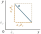
\includegraphics[scale=1]{figures/ch_01/fig_1_12.pdf}
		\caption[]{Typical crystal structures: (a) --- base-centered (BaseC); (b) --- body-centered (BC); (c) --- face-centered (FC).}
		\label{fig:1_12}
	\end{center}
	\vspace{-0.7cm}
\end{figure}

\textbf{A lattice with a basis.} Not every type of lattice may be obtained by translation of a single site. Figure \ref{fig:1_13} shows a two-dimensional lattice with a general-type basis. It may easily be seen that it is impossible to describe the unit cell of such a lattice in terms of a single-site unit cell. Such a lattice may be imagined as consisting of two Bravais lattices, $1$ and $2$, each determined by the basis vectors $\vec{a}$ and $\vec{b}$ and inserted into each other. The relative displacement of the lattices is described by an additional basis vector $\vec{A}$. The number of such basis vectors may be arbitrary.

\begin{figure}[t]
	\begin{center}
		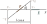
\includegraphics[scale=0.95]{figures/ch_01/fig_1_13.pdf}
		\caption[]{Two-dimensional lattice with a basis: $\vec{A}$ --- basis vector.}
		\label{fig:1_13}
	\end{center}
	\vspace{-0.7cm}
\end{figure}

The lattice of this type is termed the \textit{lattice with a basis}. It may be built with the aid of the same translations as can be used to build any of the Bravais lattices that make it up. However, in this case
we shall have to translate not one site but several sites---the \textit{basis}, defined by the totality of the basis vectors. Thus, the two-dimensional lattice shown in \fig{1_13} may be obtained by a translation of the basis made up of two sites: $0$ and $0'$. An example of a three-dimensional lattice with a basis is the diamond lattice shown in \fig{1_14}(a). It maybe obtained by inserting one FCC (face-centered
cubic) lattice into another FCC lattice displaced along the space diagonal by one-fourth of its length. Figure \ref{fig:1_14}(b) shows a tetrahedron designated by a dotted line in \fig{1_14}(a). It may be seen from \fig{1_14}(b) that in the diamond lattice every atom is surrounded by four nearest neighbours in the apexes of the tetrahedron whose edge is $a/2$.

\begin{figure}[t]
	\begin{minipage}[t]{0.6\linewidth}
		\begin{center}
			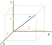
\includegraphics[scale=0.9]{figures/ch_01/fig_1_14.pdf}
			\caption[]{Diamond lattice: (a) --- spatial arrangement of atoms in the lattice; (b) --- tetrahedral pattern of atoms in the lattice.}
			\label{fig:1_14}
		\end{center}
	\end{minipage}
	\hfill{ }%\hspace{-0.1cm}
	\begin{minipage}[t]{0.33\linewidth}
		\begin{center}
			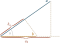
\includegraphics[scale=0.92]{figures/ch_01/fig_1_15.pdf}
			\caption[]{Indices of a crystal lattice site.}
			\label{fig:1_15}
		\end{center}
	\end{minipage}
\vspace{-0.3cm}
\end{figure}

\section{Notation to describe sites, directions, and planes in a crystal}\label{sec:1_9}

Let us mention briefly the notation conventionally used to describe sites, directions and planes in a lattice, the \textit{Miller indices}.

\textbf{Site indices.} The position of any lattice site relative to the chosen origin of coordinates is defined by three of its coordinates (\fig{1_15}): $x, y, z$. These coordinates may be expressed in the following form:
\begin{equation*}
	x = ma,\quad y = nb,\quad z = pc
\end{equation*}

\noindent
where $a, b, c$ are the lattice parameters, and $m, n, p$ are integers.

Should we use lattice parameters as units of length along the respective axes we would obtain the lattice coordinates simply in the form of numbers $m, n, p$. These numbers are termed \textit{site indices} and are written in the form $[[mnp]]$. For a negative index the minus sign is written above the index. For instance, for a site with coordinates $x=-2a, y =-lb, z=3c$ the indices are written in the form $[\bar{21}3]$.

\textbf{Indices of direction.} To describe a direction in a crystal a straight line passing through the origin is chosen. The position of this is uniquely defined by the indices of the first site through which it passes (\fig{1_15}). Therefore the indices of the site are at the same time the indices of the direction. The usual notation for a direction is $[mnp]$. The indices of direction are, by definition, the three smallest integers that describe the position of the site nearest to the origin which lies on the given direction. For instance, the indices of the direction that passes through the origin and the site $[[435]]$ are $[435]$. Figure \ref{fig:1_16} shows the principal directions (crystallographic orientations) in a cubic crystal and their notation.

\begin{figure}[t]
	\begin{center}
		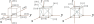
\includegraphics[scale=1.1]{figures/ch_01/fig_1_16.pdf}
		\caption[]{Indices of principal directions in a cubic crystal.}
		\label{fig:1_16}
	\end{center}
	\vspace{-0.7cm}
\end{figure}

\begin{figure}[t]
	\begin{center}
		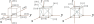
\includegraphics[scale=1.0]{figures/ch_01/fig_1_17.pdf}
		\caption[]{Indices of principal planes in a cubic crystal.}
		\label{fig:1_17}
	\end{center}
	\vspace{-0.7cm}
\end{figure}

\textbf{Plane indices.} The position of a plane is defined by the choice of three sections $A, B, C$ it cuts off when it intersects with the three coordinate axes. The procedure of finding the indices of such a plane is as follows.

The sections $ABC$ are expressed in axial units and the reciprocal quantities are written as $1/A, 1/B, 1/C$. A common denominator is found for all the three fractions. Suppose it is $D$. Then the integers $h=D/A, k=D/B, I=D/C$ will be the plane indices. They are written in the form $(hkl)$.

Determine, for example, the indices of a plane that cuts off the sections $A=1/2, B=2, C=1/3$ on the $x,y,z$ axes respectively. The ratios $1/A \div 1/B \div 1/C = 1/(1/2) \div 1/2 \div 1/(1/3) = 2 \div
1/2 \div 3$. The common denominator is $D=2$. The indices of the plane are $h=2/(1/2)=4, k=2/2=1, l=3/(1/2)=6$. The plane is denoted $(416)$. Figure \ref{fig:1_17} shows the principal planes of the cubic lattice.

It may easily be shown that in a cubic crystal the distances between the planes belonging to a given family may be expressed with the aid of the indices of these planes in the following way:
\begin{equation}\label{eq:1_17}
	d = \frac{a}{\sqrt{h^2 + k^2 + l^2}}
\end{equation}

\noindent
where $a$ is the lattice parameter. This formula shows that the greater are the plane indices the shorter is the distance between the planes.

To denote the planes in a hexagonal crystal a four-axis coordinate system is used (\fig{1_18}): three axes $(a_1, a_2, a_3)$ make angles of \ang{120} with one another and lie in the base of a hexagonal prism, the fourth axis, $c$, being perpendicular to the base plane. Every plane is denoted by four indices: $hkil$. The additional label $i$ occupies the third place and is calculated with the aid of $h$ and $k$: $i=-(h+k)$. The base plane parallel to the axes $a_1, a_2, a_3$ has the indices $(0001)$. The planes parallel to the lateral faces of the prism have indices of the $(1010)$ type. There are three such planes (not parallel to one another). They are termed \textit{first-order planes}.

\begin{figure}[t]
	\begin{center}
		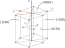
\includegraphics[scale=1.0]{figures/ch_01/fig_1_18.pdf}
		\caption[]{Indices of principal planes in a hexagonal crystal.}
		\label{fig:1_18}
	\end{center}
	\vspace{-0.7cm}
\end{figure}

\section{Classification of solids based on the nature of bonds}\label{sec:1_10}

The nature of the crystal structure is primarily dictated by the nature of bonding forces acting between the structural particles (atoms, ions, molecules) which make up the solid. In accordance with the five existing types of bonds there are five principal types of crystal lattices: \textit{ionic}, or \textit{coordination}, \textit{lattices}, with the ionic bond playing the main part; \textit{molecular lattices}, with the van der Waals forces mainly responsible for the bonding; \textit{atomic lattices}, with bonds of a distinctly covalent type; \textit{metallic lattices}, with characteristic metallic bonds; and lattices with the \textit{hydrogen bond}.

Let us analyze from this viewpoint the crystal structure of chemical elements and of typical chemical compounds (see Appendix \sect{A_iv}, Table~\ref{table:A_1}).

The chemical elements may be roughly divided into four classes according to the type of crystal structure. The analysis may best be started with Class IV.

\textbf{Class IV.} This class includes all the inert gases. In the process of compression and crystallization of these gases only comparatively weak van der Waals forces act between the atoms, which have spherically symmetrical electron shells. Acted upon by these forces the symmetrical atoms draw together to form a most tightly packed face-centered cubic lattice. Every atom is surrounded by $12$ nearest neighbours. The number of nearest neighbours is usually termed the \textit{coordination number} of the lattice.

\textbf{Class III.} The Class III includes silicon and carbon from the short periods of the Mendeleev periodic table, germanium and tin from Group IVB, and all the elements from Groups VB, VIB, VIIB.

The crystallization of the elements of those classes proceeds in conformity with the ($8-N$)-rule: every atom in the lattice is surrounded
by $8-N$ nearest neighbours, $N$ being the number of the group to which the element belongs. Thus diamond, silicon, germanium and gray tin are elements of Group IV of the Periodic Table. Therefore the coordination number of their lattices should be $8-4=4$. They all do have a tetrahedral lattice in which every atom is surrounded by $4$ nearest neighbours, as is shown in \fig{1_19}(a). Phosphorus, arsenic, antimony and bismuth belong to Groug V. Their coordination number is $8-5=3$. Every atom has $3$ nearest neighbours lying in a plane, as shown in \fig{1_19}(b). Their lattice has a laminate structure, with the atomic layers bonded by van der Waals forces.

\begin{figure}[t]
	\begin{center}
		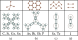
\includegraphics[scale=1.0]{figures/ch_01/fig_1_19.pdf}
		\caption[]{Crystal structure of chemical elements crystallizing in accordance with the $(8-N)$-rule: (a) --- elements of Group IVB; (b) --- elements of Group VB; (c) --- elements of Group VIB, (d) --- elements of Group VIIB.}
		\label{fig:1_19}
	\end{center}
	\vspace{-0.7cm}
\end{figure}

Selenium and tellurium belong to Group VI and have a coordination number $2$. Their atoms form long spiral-shaped chains with each atom having two nearest neighbours [\fig{1_19}(c)]. The chains are bonded by van der Waals forces. Lastly, iodine belongs to Group VII [\fig{1_19}(d)] and has a coordination number $1$. The atoms in the iodine lattice are arranged in pairs bonded by van der Waals forces. This explains the high volatility of iodine.

Such nature of the crystal structure of chemical elements whose crystallization conforms to the $(8-N)$-rule is quite understandable. The atoms of Group IV elements have $4$ electrons in their outer shell. They lack $4$ additional electrons to make up a stable $8$-electron configuration. They make up the deficit by exchanging electrons with $4$ nearest neighbours, as shown in \fig{1_19}(a), forming a strong covalent bond with each of them. Accordingly, every atom in the crystal lattice of those elements has $4$ nearest neighbours. In the same way the electron shells of Groups V, VI, VII are completed to contain $8$ electrons.

\begin{figure}[t]
	\begin{center}
		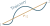
\includegraphics[scale=1.0]{figures/ch_01/fig_1_20.pdf}
		\caption[]{Structure of quartz \ce{Si02} crystal.}
		\label{fig:1_20}
	\end{center}
	\vspace{-0.7cm}
\end{figure}

Many chemical compounds crystallize in crystals with covalent bonds. Quartz \ce{SiO2} may serve as a typical example. In the quartz crystal every silicon atom is surrounded by a tetrahedron of oxygen atoms (\fig{1_20}) bonded to the silicon atom by covalent bonds. Every oxygen atom is bonded to two silicon atoms thereby joining two tetrahedrons. In this way a three-dimensional net of \ce{Si-O-Si} bonds is formed, and the hardness and the melting point of the resulting crystal are high.

It may be of interest to note that the \ce{Si-O-Si} bonds may be arranged into a one-dimensional chain. Such compounds described by the common formula
\begin{figure}[h]
	\begin{center}
		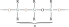
\includegraphics[scale=0.95]{figures/ch_01/chemical_formula_quartz.pdf}
	\end{center}
	\vspace{-0.7cm}
\end{figure}

\noindent
where $R$ is an arbitrary organic group, are termed \textit{silicones}. The number $n$ in a chain may be as high as several million. The chains may be joined together with the aid of the lateral groups $R$. In this way new materials, silicone resins, are formed. Because of the high strength of the \ce{Si-O-Si} bonds and of the high flexibility of silicone chains such resins retain their properties at much lower and much higher temperatures than natural rubbers. This fact enables them to be used for thermal shielding of space ships and aircraft, as well as in extreme arctic conditions.

\textbf{Class I.} This is the most populated class which contains metals. Since metallic lattices are made up not of atoms but of ions, having the spherical symmetry of the atoms of inert gases, it is to be expected that metals too should crystallize into the same tightly packed lattices as the inert gases. Indeed, the following three types of crystal lattices are characteristic for metals: the face-centered cubic lattice with the coordination number $12$ (see \fig{1_12}), the hexagonal
close-packed (HCP) lattice with the coordination number $12$ (see
\fig{1_18}) and the body-centered cubic lattice with the coordination number $8$ (see \fig{1_12}]. The latter is the least closely packed metal lattice.

\textbf{Class II.} The chemical elements belonging to Class II are in a sense intermediate between metals and the Class III elements, which crystallize in conformity with the $(8-N)$-rule. For instance, the Group IIB elements \ce{Zn}, \ce{Cd} and \ce{Hg} are metals and one would expect them to have a typically metallic lattice with a high coordination number. Actually, \ce{Zn} and \ce{Cd} crystals are a special modification of the compact hexagonal lattice in which every atom has $6$ nearest neighbours instead of $12$, as required by the $(8-N)$-rule. These atoms occupy the base plane. In the case of mercury the $(8-N)$-rule is observed even more strictly: its crystal structure is a simple rhombohedral in which every atom is surrounded by $6$ nearest neighbours. Boron---an element of Group IIIB---has a lattice that may be described as a deformed lattice with $5$ nearest neighbours. This too agrees with the $(8-N)$-rule.

\begin{figure}[t]
	\begin{center}
		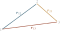
\includegraphics[scale=0.95]{figures/ch_01/fig_1_21.pdf}
		\caption[]{Structure of rock salt \ce{NaCl} crystal.}
		\label{fig:1_21}
	\end{center}
	\vspace{-0.75cm}
\end{figure}

The ionic bond, as was stated above, plays one of the main parts in the world of inorganic compounds, in particular, in numerous ionic crystals typically represented by the rock salt crystal \ce{NaCl} (\fig{1_21}). In such crystals it is impossible to pick out single molecules. The crystal should be regarded as a closely packed system of positive and negative ions whose positions alternate so that the electrostatic attraction between the nearest neighbours would be at its maximum. With the most favourable relation between the radii of the positive (\ce{M+}) and the negative (\ce{X-}) ions which exists in the \ce{NaCl} crystal the ions ``touch'' one another [\fig{1_22}(a)] and the closest possible packing is achieved, in which every ion is surrounded by $6$ nearest neighbours of the opposite charge. When the ratio of the radii of the ions \ce{M+} and is less favourable [\fig{1_22}(b,c)] crystal structures with other coordination numbers, $4$ or $8$, are formed.

\begin{figure}[t]
	\begin{center}
		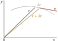
\includegraphics[scale=1.1]{figures/ch_01/fig_1_22.pdf}
		\caption[]{Effect of relative dimensions of ions on their packing in the lattice.}
		\label{fig:1_22}
	\end{center}
	\vspace{-0.7cm}
\end{figure}

Ionic compounds of the \ce{MX2} type, such as \ce{CaCl2} and \ce{Na20}, have still more complex lattices. But the principle upon which they are built remains the same: the ions are packed so as to be surrounded by ions of the opposite sign in accordance with the formula of the compound and the ratio of their radii.

Finally, let us consider crystals featuring the hydrogen bond. A typical representative of such crystals is ice. Figure \ref{fig:1_23}(a) shows a two-dimensional diagram of the arrangement of water molecules in an ice crystal: each molecule is surrounded by four nearest neighbours a distance $r_{\ce{OH}}=\SI{2.76}{\angstrom}$ away from it with whom it forms hydrogen bonds. In space the molecules occupy the vertices of a regular tetrahedron [\fig{1_23}(b)]. The combination of such tetrahedra forms the regular crystal structure of ice [\fig{1_23}(c)]. The structure is very loose and this is the cause of the abnormally low density of ice. Upon melting, some ($\sim 15\%$) of the hydrogen bonds are disrupted and the packing density of the water molecules rises somewhat with the resultant rise in the density of water: the density of ice at \SI{0}{\degreeCelsius} is \SI{916.8}{\kilo\gram\per\metre\cubed}, and the density of water at this temperature is \SI{999.87}{\kilo\gram\per\metre\cubed}.

It may be of interest to note that if there was no hydrogen bond the melting point of ice would be \SI{-100}{\degreeCelsius} instead of \SI{0}{\degreeCelsius}.

\begin{figure}[t]
	\begin{center}
		\includegraphics[scale=1.0]{figures/ch_01/fig_1_23.pdf}
		\caption[]{Crystals with hydrogen bond: (a) --- plane diagram of arrangement of water molecules in an ice crystal; (b) --- spatial arrangement of water molecules in an ice crystal; (c) --- crystal structure of ice.}
		\label{fig:1_23}
	\end{center}
	\vspace{-0.7cm}
\end{figure}

It should finally be stressed again that the hydrogen bond plays an extremely important part in vital biological compounds: protein molecules owe their helical shape exclusively to the hydrogen bond; the same type of bonds holds together the double helixes in the DNA. ``It is no exaggeration to claim that life on our planet would have assumed radically different forms---if any at all---were hydrogen bonding not present in water and in the proteins and nucleic acids that compose living cells and that transmit hereditary traits''\footnote{G. C. Pimentel and R. D. Spratley, \textit{Chemical Bonding Clarified Through
Quantum Mechanics}, Holden-Day, San Francisco (1969), p. 261.}.

Table \ref{table:A_2} of Appendix \ref{sec:A_iv} shows the general classification of solids. The upper left corner contains typical metals with collectivized electrons (silver, copper) and the upper right corner typical valence crystals with distinctly localized electron bonds. The extreme righthand part contains crystals with van der Waals bonds. Such elements as silicon and germanium occupy an intermediate position between the metals and the valence crystals. At absolute zero they are typical valence crystals; however, as temperature rises the valence bond is gradually disrupted and they begin to exhibit metallic properties. Such solids as sulphur, phosphorus, and selenium occupy an intermediate position between the valence crystals and crystals with the van der Waals bond.

The lower left corner of the diagram contains alloys of the \ce{NiCu} type with the characteristic metallic bond and the lower right corner ---ionic crystals (sodium chloride). Intermediate positions between them are occupied by numerous intermetallic compounds of the \ce{Mg3Sb2} type featuring the ionic bond (\ce{Mg3Sb2} corresponds to a \ce{Mg^{+2}-Sb^{-3}} compound). Intermediate position between the ionic and the valence crystals is occupied by such compounds as \ce{SiO2} and \ce{SiC}, with bonds of partially ionic nature made possible because of electron displacement. Compounds of the \ce{FeS} and the \ce{TiO2} (titanium dioxide) type occupy an intermediate position between ionic crystals and crystals with the van der Waals bond.

There are a great many crystals in which ionic or covalent bonds act in atomic planes while the bonds between the planes are of the van der Waals type.

\section{Polymorphism}\label{sec:1_11}

Some solids have two or more crystal structures each of which is stable in an appropriate range of temperatures and pressures. Such structures are termed \textit{polymorphic modifications}, or \textit{polymorphs},
and the transition from one modification to another, \textit{polymorphic
transformation}.

It is the practice to denote polymorphic modifications by Greek letters: the modification stable at normal and lower temperatures is denoted by \ce{\alpha}; modifications stable at higher temperatures are denoted by the letters \ce{\beta}, \ce{\gamma}, \ce{\delta}, etc. The polymorphism of tin may serve as a classical example. Below \SI{13.3}{\degreeCelsius} the stable modification of tin is \ce{\alpha-Sn}, which has a tetragonal cubic lattice of the diamond type. This is the so-called gray tin. It is brittle and may easily be ground to powder. Above \SI{13.3}{\degreeCelsius} \ce{\alpha-Sn} transforms into \ce{\beta-Sn}, which has a body-centered tetragonal lattice. This is the familiar white metallic tin, a rather ductile metal. The transformation from \ce{\beta-Sn} to \ce{\alpha-Sn} is accompanied by a considerable increase in specific volume (by about 25\%). Long ago when many things were made of tin, the perplexing phenomenon of growing bulges on them and their subsequent destruction following excessive cooling was attributed to a mysterious metal disease, the ``tin plague''.

Many other chemical elements also exhibit polymorphism: carbon, iron, nickel, cobalt, tungsten, titanium, boron, berillium, and others, as well as many chemical compounds and alloys.

An interesting and a practically important case of polymorphism is that of carbon, which exists in the forms of diamond and graphite.

This case deserves a more detailed study. In the diamond lattice every atom is surrounded by $4$ nearest neighbours occupying the vertices of a tetrahedron (see \fig{1_14}) with whom it is bonded by strong covalent forces. The length of the bond is \SI{1.544}{\angstrom} and the energy per bond is about \SI{3.5e5}{\joule\per\mole}.

\begin{figure}[t]
	\begin{center}
		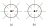
\includegraphics[scale=1.0]{figures/ch_01/fig_1_24.pdf}
		\caption[]{Crystal structure of graphite.}
		\label{fig:1_24}
	\end{center}
	\vspace{-0.7cm}
\end{figure}

The graphite lattice is of the pattern characteristic of the Group VB element lattices: the carbon atoms form two-dimensional layers in which every atom is surrounded by $3$ nearest neighbours with whom it is bonded by covalent bonds (\fig{1_24}). The length of the bond is $r_{01}=\SI{1.42}{\angstrom}$, that is, less than in the diamond lattice, therefore the former is stronger. The distance between the layers is much greater than the length of the \ce{C-C} bond, being equal to $r_{02}=\SI{3.6}{\angstrom}$. Only weak van der Waals forces can act at such great distances and the layers are held together by them. The energy of this bond is \SIrange{4e3}{8e3}{\joule\per\mole}.

Such a great difference in the nature of the bonding forces in the diamond and graphite structures should evidently manifest itself in a great difference in their properties, which is actually the case. Graphite slides easily along the planes held together by weak van der Waals forces. Therefore it is used to advantage in making ``lead'' pencils and as dry lubricant. The electrons in diamond are held securely between the atoms forming bonds. Light of the visible part of the spectrum is unable to knock out such electrons and therefore is not absorbed in diamond. Because of this diamond is an ideal transparent crystal unable to conduct electric current (a dielectric). In graphite one of the four valence electrons of the carbon atom is actually collectivized by the atoms forming the layer. Such electrons can easily be moved by the action of an external electric field, making graphite a two-dimensional conductor. The presence of mobile electrons explains light absorption (the gray colour of graphite) and its characteristic metallic glitter.

In normal conditions graphite is a somewhat more stable modification than diamond, although the difference in the energies of those modifications is quite small---of the order of \SI{2e3}{\joule\per\mole}:
\begin{equation*}
	\ce{C \text{(diamond)} -> C \text{(graphite)}},\quad \Delta{U} = \SI{-1.88e3}{\joule\per\mole}.
\end{equation*}

Still, such a difference is enough to bring about a sufficiently rapid transformation of diamond into graphite when heated above \SI{1000}{\degreeCelsius} in the absence of air.

The density of diamond is greater than that of graphite ($3500$ and \SI{2250}{\kilo\gram\per\metre\cubed}, respectively), which is due to a loose packing of the atomic layers in graphite. Therefore at greater pressures diamond becomes more stable and graphite less stable. At sufficiently high pressures diamond becomes more stable than graphite. In such conditions by raising the temperature to increase the mobility of the carbon atoms we may bring about the transformation of graphite into diamond.

The conditions for such transformation to proceed at a practical rate were calculated by the Soviet physicist O. I. Leipunskii. He writes: ``Firstly, graphite should be heated to at least \SI{2000}{\degreeCelsius} for the carbon atoms to be able to move from place to place. Secondly, it must be subjected to very high pressure, not less than \SI{60000}{\atm}''\footnote{Leipunskii, O. I.: Quoted from I. I. Shafranovskii, \textit{Diamonds}, ``Nauka'', Moscow (1964).}. These conditions were first achieved by the scientists of the General Electric Research and Development Center, who in 1954 succeeded in producing the first synthetic diamonds in the form of dark unsightly crystals, the largest being \SI{1.5}{\milli\metre} long. Subsequently, the synthesis of diamonds was mastered in Sweden, the Netherlands, and Japan.

In the Soviet Union the production of synthetic diamonds on a comercial scale began in 1961. The pressure in the process is of the order of \SI{100000}{\atm} and the temperature about \SI{2000}{\degreeCelsius}. Synthetic diamonds produced by this process are harder and stronger than natural diamonds and their industrial use is about 40\% more efficient than that of natural ones.

Another material of extreme hardness had been synthesized in a process similar to that of the diamond---the cubic boron nitride \ce{BN}, which became known as \textit{borazon}. It is harder than diamond and may be heated up to \SI{2000}{\degreeCelsius} in atmospheric conditions. In its hexagonal modification boron nitride is similar to graphite---a white powder oily to the touch.

From the theoretical point of view all solids should exhibit polymorphism provided the range of their stability is not limited by the processes of melting and sublimation. The existence of polymorphism is a direct consequence of the variation of the strength and the nature of the bonds in the crystal lattice caused by the changes in intensity of atomic motion and in the distance between them as a result of heating or of application of external pressure to the crystal. Close to absolute zero the stable structure should be that with the strongest bonds possible for the given atomic ensemble. In the case of tin, which belongs to Group IV of the Mendeleev periodic table, such structure is the diamond structure, in which every atom is bonded to $4$ nearest neighbours by strong covalent bonds. However, as the temperature is raised, those bonds, because of their strict directionality and rigidity, are easily destroyed by thermal motion, and already above \SI{13.3}{\degreeCelsius} the flexible metallic structure formed with the aid of collectivized electrons becomes more favourable. This bond has its own stable crystal structure, the tetragonal body-centred lattice.

The transition from one modification to another is accompanied by the liberation or absorption of latent heat of transformation and is therefore a phase transition of the first kind. Such a transition involves the transformation of the crystal lattice and this fact together with a low mobility of atoms in solids makes possible a practically infinitely long existence of a modification thermodynamically unstable in particular conditions. Diamond which can exist ages without turning into graphite---the stable modification in normal conditions---is a striking example of this point.

Polymorphism is very important for practical purposes. Heat treatment of steels to obtain various properties, the production of stainless steels, the treatment of various alloys to obtain the necessary properties are all to a large extent based on the use of polymorphism.

\section{Imperfections and defects of the crystal lattice}\label{sec:1_12}

\textbf{Mosaic structure.} Numerous data obtained in the study of the structure of real crystals point to the fact that their internal structure is essentially not the same as that of an ideal crystal. To begin with, real crystals have a \textit{mosaic structure}: they are made up of regular blocks which are only approximately parallel to one another. The dimensions of the blocks vary from \SIrange{e-6}{e-8}{\metre} and the angles between them from several seconds to tens of minutes. Because of the different orientation of adjacent blocks there is a transition layer between them in which the lattice changes its orientation gradually from that of the first block to that of the second. Therefore in this layer the lattice is deformed as compared with that of an ideal crystal.

Lattice deformations are even greater near the grain boundaries in a polycrystal, since the orientation of adjacent grains may differ by as much as tens of degrees. The grain and block boundaries carry excess free energy, which increases the rate of chemical reactions, of polymorphic transformations, of diffusion, etc. They also serve as effective carrier scattering centres responsible for a considerable part of the solid's (metal or semiconductor) electrical resistance.

\textbf{Frenkel defects.} The distribution of energy among the atoms of a solid is very nonuniform, as is the case with the molecules of a gas or liquid. At any temperature there are atoms in the crystal whose energy is many times greater or less than the average energy corresponding to the law of equipartition of energy. The atoms that at a given instant of time have enough energy can not only move a considerable distance away from their position of equilibrium, but can also surmount the potential barrier set up by the neighbouring atoms and move over to new neighbours, to a new cell. Such atoms acquire the capability, so to say, to ``evaporate'' from their lattice sites and to ``condense'' in its internal cavities, or interstitials [\fig{1_25}(a)]. This process results in the creation of a vacant site (a \textit{vacancy}) and of an atom in the interstitial position (a \textit{displaced atom}). Such lattice defects are termed \textit{Frenkel defects}.

\begin{figure}[t]
	\begin{center}
		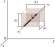
\includegraphics[scale=1.1]{figures/ch_01/fig_1_25.pdf}
		\caption[]{Crystal lattice defects: (a) --- Frenkel defects; (b), (c) --- Schottky defects.}
		\label{fig:1_25}
	\end{center}
	\vspace{-0.7cm}
\end{figure}

Calculation shows the equilibrium concentration of interstitial atoms $\ab{n}{F}$ at a given temperature to be
\begin{equation}\label{eq:1_18}
	\ab{n}{F} = A N \exp\parenthesis{-\frac{\ab{E}{F}}{\ab{k}{B}T}}
\end{equation}

\noindent
where $\ab{E}{F}$ is the formation energy of the interstitial whose order of magnitude is several electron volts, $N$ is the number of sites in the given volume, $A$ is an integer (usually about $1$) indicating the
number of identical interstitial positions per one lattice atom, and $\ab{k}{B}$ is the Boltzmann constant.

Both the interstitial atoms and the vacancies do not remain localized in one place but diffuse through the lattice. The diffusion of a displaced atom proceeds by the motion of this atom from one interstitial position to another, and the diffusion of a vacancy by a relay process in which the vacancy is filled by neighbouring atoms [\fig{1_25}(a)]: when atom $2$ moves into vacancy $1$ the vacancy moves over to site $2$, when atom $3$ moves to the now vacant site $2$ the vacancy moves to site $3$, etc.

\textbf{Schottky defects.} In addition to internal evaporation there is also a possibility of a partial or even complete evaporation of an atom from the surface of a crystal. Complete evaporation means that the atom leaves the crystal surface and joins the vapour phase [\fig{1_25}(b)]. Partial evaporation means that the atom leaves the surface layer and arranges itself on top of it [\fig{1_25}(c)]. In both cases a vacancy is produced in the surface layer. But when an atom from the interior of a crystal occupies a vacancy, the latter is pulled into the crystal and diffuses there. Here there are no displaced atoms to correspond to the vacancies, since the latter are produced without the simultaneous transition of atoms to interstitial positions. Such vacancies are termed \textit{Schottky defects}. Calculations show the equilibrium number of vacancies $\ab{n}{Scn}$ in a crystal of $N$ sites to be
\begin{equation}\label{eq:1_19}
	\ab{n}{Scn} = N \exp\parenthesis{-\frac{\ab{E}{Scn}}{\ab{k}{B}T}}
\end{equation}

\noindent
where $\ab{E}{Scn}$ is the energy of formation of a single vacancy. It is somewhat lower than $\ab{E}{F}$. For instance, for aluminium it is equal to \SI{0.75}{\electronvolt}. Substituting this value into \eqref{eq:1_19}, we obtain $\ab{n}{Scn}\approx\SI{e18}{\per\metre\cubed}$ at $T=\SI{300}{\kelvin}$; at $T=\SI{923}{\kelvin}$, that is, close to the melting point of aluminium ($\ab{T}{m}=\SI{933}{\kelvin}$), $\ab{n}{Scn}\approx\SI{e25}{\per\metre\cubed}$.
Such values are characteristic of all metals at temperatures close to their melting points.

The energy of formation of the Frenkel defects is approximately equal to the sum of formation energies of the vacancy and the interstitial atom.

The Frenkel and Schottky defects play an important part in many processes in crystals. They act as carrier scattering centres reducing their mobility. They can also act as sources of carrier production, that is, play the role of donors and acceptors (usually the latter). They can also appreciably affect optical, magnetic, mechanical, and thermodynamic properties of crystals, especially of thin semiconducting films and fine crystalline specimens (because defect concentration in them is usually much greater than in bulk specimens).

\textbf{Impurities.} Impurities are one of the most important and most common type of detects in the structure of real crystals. Contemporary refining methods are unable to guarantee absolute purity of materials. Even the most pure materials contain up to \num{e-9} percent of impurities, which corresponds to a concentration of about \num{e17} impurity atoms per cubic metre of the material. To illustrate this degree of purity we would like to cite an equivalent example of one grain of rye contained in about $10$ tons of wheat.

The impurities contained in the crystal may, depending on their nature, be in the form of dissolved atoms or in the form of inclusions of various dimensions. In the process of dissolution the impurity atoms enter the interstitial positions between the atoms of the crystal or substitute some of them in their sites. The solid solution of the first type is termed the \textit{interstitial solution} [\fig{1_26}(a)] and that of the second the \textit{substitution solution} [\fig{1_26}(b)]. Because of a difference in the physical nature and the dimensions of the impurity atoms from the atoms of the crystal, their presence results in the deformation of the crystal lattice.

Impurities may appreciably affect chemical, optical, magnetic, and mechanical properties of solids. They are effective carrier scattering centres, being the cause of electrical resistance that does not vanish at absolute zero temperature. In semiconductor crystals the impurities create new energy levels leading to the appearance of impurity conductivity. Calculations show that a perfectly pure silicon should have a specific resistance of the order of \SI{2000}{\ohm\metre}. Active impurities contained in it in a concentration of \num{e-9} percent reduce the resistivity to several units. Technically pure germanium was for a long time regarded as a metal because its resistivity was of the same order as that of metals. Only perfect refining methods that brought impurity concentration in germanium down to \num{e-7}-\num{e-8} percent made it a typical semiconductor.

\begin{figure}[t]
	\begin{center}
		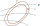
\includegraphics[scale=1.1]{figures/ch_01/fig_1_26.pdf}
		\caption[]{Deformations of crystal lattice of solid solutions: (a) --- interstitial; (b) --- substitution.}
		\label{fig:1_26}
	\end{center}
	\vspace{-0.7cm}
\end{figure}

Interesting results were obtained in the course of investigations into the properties of extremely pure metals. Thus thoroughly purified iron turned out to be chemically inert and immune to corrosion even in conditions of tropical humidity. Titanium, chromium, bismuth, tungsten, molybdenum, which had a reputation for brittleness, turned out to be ductile even in conditions of extreme cooling; tin purified to contain no more than \num{5e-6} percent impurities is so soft that it bends under its own weight like dough.

Some striking results were obtained in dehydration experiments: materials dried so as to contain negligible amounts of residual moisture change their properties in a marked degree. Thus dried oxyhydrogen gas does not explode at high temperatures; carbon monoxide does not burn in oxygen; sulphuric acid does not react with alkali metals, etc. The English chemist H. B. Baker sealed $11$ thoroughly purified individual chemical compounds in glass tubes together with phosphoric anhydride (a powerful absorber of water). The tubes were opened $9$ years later in conditions that precluded the admission of moisture. The results were startling: the boiling point of all the compounds rose appreciably. For instance, the boiling point of benzol turned out to be \SI{26}{\degreeCelsius} higher than that specified in tables, that of ethyl alcohol was \SI{60}{\degreeCelsius} higher, that of bromine was \SI{59}{\degreeCelsius} higher, and that of mercury was almost \SI{100}{\degreeCelsius} higher. Subsequent experiments carried out by other investigators substantiated those results. More than that, it was established that very dry materials not only change their boiling point but melting point and other properties as well.

Despite substantial progress in the field of production of ultrapure materials there is a growing demand for better purification methods and presently there will be a need for materials with impurity concentrations
of no more than \num{e-10}-\num{e-12} percent. This applies in the first instance to materials used for thermonuclear fusion apparatus, to microelectronics materials, as well as to materials used in other branches of industry. Such materials are not only difficult to produce but also difficult to keep pure, especially if they have to be processed before use. To illustrate how easy it is to make a mistake while working with such materials we would like to cite a case told by the well-known German physicist Werner Heisenberg. When a target was irradiated with a flux of neutrons in a mass spectrometer, gold nuclei were detected. This effect vanished after the experimenter took off and put away his gold-rimmed eyeglasses.
